% !TEX root = ../thesis-main.tex
\section{Обзор и сравнение существующих генераторов программного кода}

\subsection{Понятие генерации программного кода}

\textbf{Генерация программного кода} --- это автоматическое создание программного кода специальным приложением, при котором по заданным условиям полностью или частично формируется исходный код программы. Такое специальное приложение называется \textbf{генератором кода}. Получается, что это программа, создающая программный код.

Основной сферой применения генераторов программного кода является автоматическое тестирования компиляторов. 
С помощью них можно обнаружить незаметные ошибки которые могут влиять на работу скомпилированного этими компиляторами программного обеспечения. В сравнение были включены
несколько инструментов для тестирования компиляторов.

Также для поиска существующих аналогов был произведен поиск в поисковых системах “Google” и “Google Scholar”
по следующим ключевым словам:
\begin{itemize}
    \item “C++ program generator”
    \item “program generator”
    \item “random program generator”
    \item "java program generator"
    \item "python program generator"
\end{itemize}

В обзор не включены различные генераторы привязок к SQL таблицам
(Spring Data JPA, jOOQ и подобные), шаблоны для языков разметки
(jinja, Django Template Engine) в виду их узкой специализации.
Были получены следующие результаты, соответствующие теме дипломной работы:
% Ненумерованная формула:

% \begin{equation}
%     \begin{pmatrix} \dot{\varphi}\\ \dot{\theta} \\ \dot{\psi} \end{pmatrix}
%     = \begin{pmatrix}
%         cos(\theta)cos(\psi) & -sin(\psi) & 0 \\
%         cos(\theta)sin(\psi) & cos(\psi)  & 0 \\
%         -sin(\theta)         & 0         &  1
%     \end{pmatrix}^{-1}
%     \begin{pmatrix} \omega_x\\ \omega_y \\ \omega_z \end{pmatrix}.
% \end{equation}

% Нумерованная формула:

% \begin{equation}
%     i^2 = -1.
%     \label{eq:my_ref}
% \end{equation}

% Тест ссылки на формулу \ref{eq:my_ref}.

\subsection{Automated C++ Program Generator using English Language Interface}

В статье \cite{pg-eli} описана программа, генерирующая код на C++ с помощью описания на английском языке.
Из описания выделяются ключевые слова и параметры, которым сопоставляются один из множества поддерживаемых шаблонов и алгоритмов, в которые передаются параметры.
Поддерживаются арифметические операции, числовые алгоритмы, строковые алгоритмы, алгоритмы над последовательностями и операции ввода-вывода.
% \begin{figure}[ht]
% \begin{center}
% \scalebox{0.4}{
%    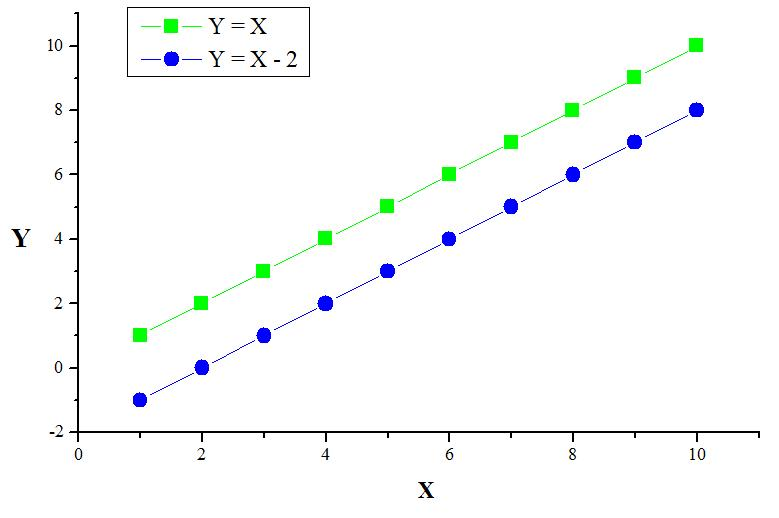
\includegraphics{images/graph.jpg}
% }

% \caption{
% \label{graph-fig}
%      Линейные функции.}
% \end {center}
% \end {figure}
% Ссылаемся на график~\ref{graph-fig}.
 
\subsection{Automatic code generation for C and C++ programming}

В статье \cite{acg-2021} описана программа, генерирующая код на C++ с помощью описания в виде блок-схем.
Элементами блок-схемы является ввод-вывод, условные ветвления и циклы.
Следствием этого является ограниченный набор поддерживаемых операций,
но в то же время за счет низкоуровневого интерфейса данная программа может генерировать более сложные программы.

\subsection{Csmith}

Csmith --- инструмент для генерации случайных программ на языке программирования C в соответствии со стандартом C99.
Используется в тестировании компиляторов, благодаря нему получилось найти более 400 ошибок в компиляторах языка C которые не были известны до этого.
Также поддерживает генерацию кода на C++. \cite{csmith}
% В работах иногда приводят фрагменты кода:
% 
% \begin{minted}{kotlin}
% fun main() {
%     val name = "stranger"
%     println("Hi, $name!")
%     print("Current count:")
%     for (i in 0..10) {
%         print(" $i")
%     }
% }
% \end{minted}


\subsection{Liveness-Driven Random Program Generation (ldrgen)}

Проект, основанный на идеях Csmith, также созданный для тестирования компиляторов.
Основная идея - уменьшение количества “мертвого кода” при генерации,
что позволяет добиться большего количества инструкций на строку кода и,
соответственно, генерировать более компактные программы для тестирования. \cite{ldrgen}


\subsection{Yarpgen}

Инструмент для генерации случайных программ на языке C для тестирования компиляторов.
Для тестирования вычисляется хэш всех значений глобальных переменных программы после ее запуска.
По сравнению с Csmith код, сгенерированный Yarpgen, более похож на написанный человеком,
так как в некоторых случаях сначала генерируется более высокоуровневая модель,
которая затем наполняется случайными данными.
Также гарантируется отсутствие неопределенного поведения у сгенерированных программ. \cite{yarpgen}

\subsection{Deepsmith}

Инструмент для генерации программ для библиотеки OpenCL на основе машинного обучения.
Сгенерированный код похож на написанный человеком так как модель обучена на open-source коде с github.
\cite{deepsmith}

\subsection{SL Random Program Generator}

Инструмент для генерации случайных программ на языке Python. Можно настраивать количество инструкций и используемые в выражениях операторы. 
Имеется веб-версия, гле также можно найти исходны код и грамматику. \cite{sl}

\subsection{Pyfuzz}

Инструмент для генерации случайных программ на языке Python. Используется для тестирования
инструментов компиляции и JIT-интерпретации Python-кода. \cite{pyfuzz}

Имеется веб-версия \cite{pyfuzz-web}

\subsection{Сравнительный анализ найденных инструментов и статей}

Сравнение аналогов будет проведено по следующим критериям:
\begin{itemize}
    \item “Читаемость кода”, то есть похож ли сгенерированный код на написанный человеком
    \item Возможность расширения на разные языки программирования (расширяемость)
    \item Наличие интерфейса для взаимодействия
    \item Возможность настройки параметров генерации
    \item Поддержка рандомизации, в частности, возможность настроить начальное значение для генератора случайных чисел
\end{itemize}

Для статей ответы критерии будут проверяться из описания, так как код реализации отсутствует в открытом доступе.

Сравнение по данным критериям представлено в Таблице \ref{table-smth}.

\begin{table}[ht]
\begin{threeparttable}[t]
\begin{tabular}{p{5.1em}|m{4em}m{5em}m{4em}m{4em}m{4em}}
    Инструмент                                                       & Чита-\newline емость & Расширя-\newline емость & Интер-\newline фейс & Настройка параметров & Рандо-\newline мизация \\
    \hline                                                                                                                                                                                  \\
    Automated C++ Program Generator using English Language Interface & +                    & +                       & Natural language    & +                    & -                      \\
    \hline                                                                                                                                                                                  \\
    Automatic code generation for C and C++ programming              & +                    & +                       & Block-scheme        & +                    & -                      \\
    \hline                                                                                                                                                                                  \\
    Csmith                                                           & -                    & -                       & CLI\tnote{1}                 & +                    & +                      \\
    \hline                                                                                                                                                                                  \\
    ldrgen                                                           & -                    & -                       & CLI                 & +                    & +                      \\
    \hline                                                                                                                                                                                  \\
    Yarpgen                                                          & -                    & -                       & CLI                 & +                    & +                      \\
    \hline                                                                                                                                                                                  \\
    Deepsmith                                                        & +                    & -                       & CLI                 & +                    & -                      \\
    \hline
    SL Random Program Generator & + & - & Web & + & +/-\tnote{2}   \\
    \hline
    Pyfuzz & - & - & Web and CLI & +\tnote{3}   & +\tnote{3}  \\
    \hline
\end{tabular}
\caption{
    \label{table-smth}
    Сравнение аналогов.}
\begin{tablenotes}
 \item[1] CLI = Command Line Interface (интерфейс командной строки)
 \item[2] Отсутствует возможность задания seed для генератора случайных значений.
 \item[3] Только в CLI
\end{tablenotes}
\end{threeparttable}
\end{table}
\clearpage

\subsubsection{Результаты сравнения}

Инструменты, описанные в статьях \cite{pg-eli} и \cite{acg-2021}, имеют разный интерфейс, но оба
имеют ограниченную параметризацию и генерируют читаемый код, однако не имеют поддержки рандомизации.

Csmith, ldrgen, и Yarpgen имеют схожий функционал и недостатки, однако среди них csmith имеет наиболее
широкую степень параметризации, Yarpgen и ldrgen имеют меньшую возможность кастомизации.

Deepsmith благодаря машинному обучению генерирует код, максимально схожий с написанным человеком,
однако, по этой же причине, обладает небольшой возможностью кастомизации и не поддерживает какую-либо
рандомизацию.

SL Random Program Generator имеет удобный веб-интерфейс, но ограниченную возможность
настройки и рандомизацию, так же очень ограничено количество поддерживаемых языковых конструкций языка Python.

Pyfuzz так же имеет веб интерфейс, однако в нем совсем отсутствует возможность настройки и рандомизации.
В CLI такая возможность присутствует, однако получившиеся программы все же используются для 
тестирования компиляторов и интерпретаторов, поэтому код получется плохо читаемым для человека.